%==============================================================================
% tento soubor pouzijte jako zaklad
% this file should be used as a base for the thesis
% Autoři / Authors: 2008 Michal Bidlo, 2016 Jaroslav Dytrych
% Kontakt pro dotazy a připomínky: dytrych@fit.vutbr.cz
% Contact for questions and comments: dytrych@fit.vutbr.cz
%==============================================================================
% kodovani: UTF-8 (zmena prikazem iconv, recode nebo cstocs)
% encoding: UTF-8 (you can change it by command iconv, recode or cstocs)
%------------------------------------------------------------------------------
% zpracování / processing: make, make pdf, make clean
%==============================================================================
% Soubory, které je nutné upravit: / Files which have to be edited:
%   projekt-20-literatura-bibliography.bib - literatura / bibliography
%   projekt-01-kapitoly-chapters.tex - obsah práce / the thesis content
%   projekt-30-prilohy-appendices.tex - přílohy / appendices
%==============================================================================
\documentclass[slovak,cprint]{fitthesis} % bez zadání - pro začátek práce, aby nebyl problém s překladem
%\documentclass[english]{fitthesis} % without assignment - for the work start to avoid compilation problem
%\documentclass[zadani]{fitthesis} % odevzdani do wisu - odkazy jsou barevné
%\documentclass[english,zadani]{fitthesis} % for submission to the IS FIT - links are color
%\documentclass[zadani,print]{fitthesis} % pro tisk - odkazy jsou černé
%\documentclass[zadani,cprint]{fitthesis} % pro barevný tisk - odkazy jsou černé, znak VUT barevný
%\documentclass[english,zadani,print]{fitthesis} % for the color print - links are black
%\documentclass[english,zadani,cprint]{fitthesis} % for the print - links are black, logo is color
% * Je-li práce psaná v anglickém jazyce, je zapotřebí u třídy použít 
%   parametr english následovně:
%   If thesis is written in english, it is necessary to use 
%   parameter english as follows:
%      \documentclass[english]{fitthesis}
% * Je-li práce psaná ve slovenském jazyce, je zapotřebí u třidy použít 
%   parametr slovak následovně:
%      \documentclass[slovak]{fitthesis}

% Základní balíčky jsou dole v souboru šablony fitthesis.cls
% Basic packages are at the bottom of template file fitthesis.cls
% zde můžeme vložit vlastní balíčky / you can place own packages here

% Kompilace po částech (rychlejší, ale v náhledu nemusí být vše aktuální)
% Compilation piecewise (faster, but not all parts in preview will be up-to-date)
% \usepackage{subfiles}

% Nastavení cesty k obrázkům
% Setting of a path to the pictures
%\graphicspath{{obrazky-figures/}{./obrazky-figures/}}
%\graphicspath{{obrazky-figures/}{../obrazky-figures/}}

%---rm---------------
\renewcommand{\rmdefault}{lmr}%zavede Latin Modern Roman jako rm / set Latin Modern Roman as rm
%---sf---------------
\renewcommand{\sfdefault}{qhv}%zavede TeX Gyre Heros jako sf
%---tt------------
\renewcommand{\ttdefault}{lmtt}% zavede Latin Modern tt jako tt

% vypne funkci šablony, která automaticky nahrazuje uvozovky,
% aby nebyly prováděny nevhodné náhrady v popisech API apod.
% disables function of the template which replaces quotation marks
% to avoid unnecessary replacements in the API descriptions etc.
\csdoublequotesoff

% =======================================================================
% balíček "hyperref" vytváří klikací odkazy v pdf, pokud tedy použijeme pdflatex
% problém je, že balíček hyperref musí být uveden jako poslední, takže nemůže
% být v šabloně
% "hyperref" package create clickable links in pdf if you are using pdflatex.
% Problem is that this package have to be introduced as the last one so it 
% can not be placed in the template file.
\ifWis
\ifx\pdfoutput\undefined % nejedeme pod pdflatexem / we are not using pdflatex
\else
\usepackage{color}
\usepackage[unicode,colorlinks,hyperindex,plainpages=false,pdftex]{hyperref}
\definecolor{links}{rgb}{0.4,0.5,0}
\definecolor{anchors}{rgb}{1,0,0}
\def\AnchorColor{anchors}
\def\LinkColor{links}
\def\pdfBorderAttrs{/Border [0 0 0] }  % bez okrajů kolem odkazů / without margins around links
\pdfcompresslevel=9
\fi
\else % pro tisk budou odkazy, na které se dá klikat, černé / for the print clickable links will be black
\ifx\pdfoutput\undefined % nejedeme pod pdflatexem / we are not using pdflatex
\else
\usepackage{color}
\usepackage[unicode,colorlinks,hyperindex,plainpages=false,pdftex,urlcolor=black,linkcolor=black,citecolor=black]{hyperref}
\definecolor{links}{rgb}{0,0,0}
\definecolor{anchors}{rgb}{0,0,0}
\def\AnchorColor{anchors}
\def\LinkColor{links}
\def\pdfBorderAttrs{/Border [0 0 0] } % bez okrajů kolem odkazů / without margins around links
\pdfcompresslevel=9
\fi
\fi
% Řešení problému, kdy klikací odkazy na obrázky vedou za obrázek
% This solves the problems with links which leads after the picture
\usepackage[all]{hypcap}

% Informace o práci/projektu / Information about the thesis
%---------------------------------------------------------------------------
\projectinfo{
	%Prace / Thesis
	project=BP,            %typ práce BP/SP/DP/DR  / thesis type (SP = term project)
	year=2019,             % rok odevzdání / year of submission
	date=\today,           % datum odevzdání / submission date
	%Nazev prace / thesis title
	title.cs={Filtrovanie sieťovej prevádzky},  % název práce v češtině či slovenštině (dle zadání) / thesis title in czech language (according to assignment)
	title.en={Network traffic filtering}, % název práce v angličtině / thesis title in english
	%title.length={14.5cm}, % nastavení délky bloku s titulkem pro úpravu zalomení řádku (lze definovat zde nebo níže) / setting the length of a block with a thesis title for adjusting a line break (can be defined here or below)
	%Autor / Author
	%author={Jméno Příjmení},   % celé jméno a příjmení autora / full name and surname of the author
	author.name={Jozef},   % jméno autora / author name
	author.surname={Urbanovský},   % příjmení autora / author surname 
	author.title.p=Bc., % titul před jménem (nepovinné) / title before the name (optional)
	supervisor.name={Adrián},   % jméno autora / author name
	supervisor.surname={Tomašov},   % příjmení autora / author surname 
	supervisor.title.p=Bc., % titul před jménem (nepovinné) / title before the name (optional)
	%author.title.a=PhD, % titul za jménem (nepovinné) / title after the name (optional)
	%Ustav / Department
	department=UIFS, % doplňte příslušnou zkratku dle ústavu na zadání: UPSY/UIFS/UITS/UPGM / fill in appropriate abbreviation of the 
	% Klíčová slova / keywords
	keywords.cs={počítačové siete, monitorovanie, skenovanie, mapovanie, bezpečnosť}, % klíčová slova v českém či slovenském jazyce / keywords in czech or slovak language
	keywords.en={networks, monitoring, scanning, mapping, security}, % klíčová slova v anglickém jazyce / keywords in english
	% Abstrakt / Abstract
	abstract.cs={Táto práca sa zaoberá sieťovou aplikáciou na skenovanie siete a otvorených portov. Jej realizácia je inšipirovaná voľne dostupným programom Nmap.}, % abstrakt v českém či slovenském jazyce / abstract in czech or slovak language
	abstract.en={This project is network application for network scanning and open ports. Realization of this work is inspired by open-source program Nmap.}, % abstrakt v anglickém jazyce / abstract in english
	% Prohlášení (u anglicky psané práce anglicky, u slovensky psané práce slovensky) / Declaration (for thesis in english should be in english)
	declaration={Prehlasujem, že som tento projekt vypracovával samostatne s využitím verbálnej komunikácie spolužiakov pracujúcich na tomto projekte. Uviedol som všetky literárne pramene a publikácie z ktorých som čerpal.},
	%declaration={Hereby I declare that this bachelor's thesis was prepared as an original author’s work under the supervision of Mr. X
	% The supplementary information was provided by Mr. Y
	% All the relevant information sources, which were used during preparation of this thesis, are properly cited and included in the list of references.},
	% Poděkování (nepovinné, nejlépe v jazyce práce) / Acknowledgement (optional, ideally in the language of the thesis)
	acknowledgment={Chcel by som poďakovať za aktivitu na fóre ako spolužiakom, tak zadávateľovi tohto projektu.},
	%acknowledgment={Here it is possible to express thanks to the supervisor and to the people which provided professional help
	%(external submitter, consultant, etc.).},
	% Rozšířený abstrakt (cca 3 normostrany) - lze definovat zde nebo níže / Extended abstract (approximately 3 standard pages) - can be defined here or below
	%extendedabstract={Do tohoto odstavce bude zapsán rozšířený výtah (abstrakt) práce v českém (slovenském) jazyce.},
	faculty={FEKT}, % FIT/FEKT/FSI/FA/FCH/FP/FAST/FAVU/USI/DEF
	faculty.cs={Fakulta elektrotechniky a komunikačních technologií}, % Fakulta v češtině - pro využití této položky výše zvolte fakultu DEF / Faculty in Czech - for use of this entry select DEF above
	faculty.en={Faculty of Electrical Engineering and Communication}, % Fakulta v angličtině - pro využití této položky výše zvolte fakultu DEF / Faculty in English - for use of this entry select DEF above
	department.cs={Ústav matematiky}, % Ústav v češtině - pro využití této položky výše zvolte ústav DEF nebo jej zakomentujte / Department in Czech - for use of this entry select DEF above or comment it out
	department.en={Institute of Mathematics} % Ústav v angličtině - pro využití této položky výše zvolte ústav DEF nebo jej zakomentujte / Department in English - for use of this entry select DEF above or comment it out
}

% Rozšířený abstrakt (cca 3 normostrany) - lze definovat zde nebo výše / Extended abstract (approximately 3 standard pages) - can be defined here or above
%\extendedabstract{Do tohoto odstavce bude zapsán výtah (abstrakt) práce v českém (slovenském) jazyce.}

% nastavení délky bloku s titulkem pro úpravu zalomení řádku - lze definovat zde nebo výše / setting the length of a block with a thesis title for adjusting a line break - can be defined here or above
%\titlelength{14.5cm}


% řeší první/poslední řádek odstavce na předchozí/následující stránce
% solves first/last row of the paragraph on the previous/next page
\clubpenalty=10000
\widowpenalty=10000

\begin{document}
	% Vysazeni titulnich stran / Typesetting of the title pages
	% ----------------------------------------------
	\maketitle
	% Obsah
	% ----------------------------------------------
	\setlength{\parskip}{0pt}
	
	{\hypersetup{hidelinks}\tableofcontents}
	
	% Seznam obrazku a tabulek (pokud prace obsahuje velke mnozstvi obrazku, tak se to hodi)
	% List of figures and list of tables (if the thesis contains a lot of pictures, it is good)
	
	\ifczech
	\renewcommand\listtablename{Seznam tabulek}
	\fi
	\ifslovak
	\renewcommand\listtablename{Zoznam tabuliek}
	\fi
	% \listoftables 
	
	\ifODSAZ
	\setlength{\parskip}{0.5\bigskipamount}
	\else
	\setlength{\parskip}{0pt}
	\fi
	
	% vynechani stranky v oboustrannem rezimu
	% Skip the page in the two-sided mode
	\iftwoside
	\cleardoublepage
	\fi
	
	% Text prace / Thesis text
	% ----------------------------------------------
	%=========================================================================

\chapter{Úvod}
Táto práca je dokumentáciou k samostatnému projektu z predmetu \emph{Aplikovaná kryptografie}. Samostatný projekt sa zaoberá filtrovaním sieťovej prevádzky v systéme GNU/Linux. Cieľom tohto projektu je programovo realizovať aplikáciu, ktorá má na starosť filtrovať zašifrovanú sieťovú prevádzku. Aplikácia má vytvárať štatistiky o type a množstve šifrovaných dát v sieti a ponúknuť možnosť si ich zobraziť v grafickej forme. 

\chapter{Analýza}
V~tejto kapitole je analyzovaná problematika a spôsob riešenia, ktorý je použitý pri tvorbe tejto programovej aplikácie. Dokumentácia predpokladá, že čitateľ pozná koncepty TCP/IP sieťového modelu a Linuxového jadra.

\section{Firewall a filtrovanie}
\emph{Firewall} možno označiť ako ľubovoľné sieťové zariadenie, alebo sieťovú aplikáciu, ktorá slúži k riadeniu sieťovej prevádzky medzi logicky oddelenými sieťami. Podstata firewallu je v predefinovaných pravidlách pre jednotlivé pakety a toky na základe informácii z rôznych vrstiev ISO/OSI modelu. Firewally je možné rozdeliť do nasledujúcich kategórii na základe vývoja počítačových sietí. 

\begin{itemize}
	\itemsep0em 
	\item Paketový filter
	\item Aplikačný filter
	\item Stavový paketový filter
	\item Stavový paketový filter s kontrolou protokolov ľubovoľných vrstiev ISO/OSI modelu
\end{itemize}

\cite{Oppliger1997}

\section{Implementácia v Linuxovom jadre}
Moderné Linuxové jadro ponúka granulárnu kontrolu rôznych implementácii firewallu pre filtrovanie sieťových paketov. Práca rozoberá staršiu implementáciu filtrovania pomocou \emph{iptables}, nástupcu vo forme \emph{nftables} a aj firewall následujúcej generácie známy ako \emph{bpfilter} \cite{manpages}.

\subsection{netfilter}
\emph{netfilter} je možné reprezentovať ako framework Linuxového jadra, slúžiacia pre filtrovanie paketov, preklad sieťových adries alebo preklad sieťových portov. Jeho hlavnú úlohu v jadre plnia hooky, ktoré dovolujú meniť správanie jadra ostatným modulom. Každý paket prechádzajúci kernel prejde cez sadu hookov, ktoré môže zaregistrovať predurčený modul jadra cez callback a následne zareagovať spustením obslužnej procedúry. Netfilter hooking systém obsahuje moduly jadra ako napríklad \texttt{ip\_tables}, \texttt{ip6\_tables}, \texttt{arp\_tables} a \texttt{ebtables}, ktoré možno reprezentovať ako tabuľky pre definíciu pravidiel firewallu \cite{netfilter, manpages}. 

\subsection{iptables}
Modul jadra \texttt{ip\_tables} spolu s userspace programom \texttt{iptables} slúži na manipuláciu s tabuľkami \emph{Xtables}, ktoré umožnujú združovať sady pravidiel do reťazcov. Reťazce následne definujú jednotlivé pravidlá pre pakety a sú spracovávané sekvenčne. Pravidlá umožnujú ovyplvňovať priechod sieťovým zásobníkom, kde každý paket musí prejsť aspoň jednou tabuľkou.
\cite{iptables_le, netfilter, manpages}
\begin{figure}[h]
	\centering
	\label{iptables}
	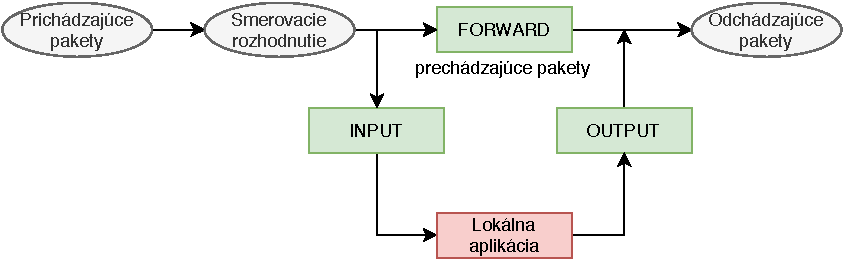
\includegraphics[scale=1.07]{obrazky-figures/iptables.pdf}
	\caption{Základné reťazce \emph{iptables} obsiahnuté v \emph{netfilteri} v tabuľke filter}
\end{figure}
                                                                                              
\emph{iptables} ponúka konfiguráciu \emph{netfilteru} ako stavového paketového filtra možného filtrovať sieťovú prevádzku na základe typu protokolu, zdrojovej a cieľovej adresy, zdrojového a cieľového portu, znalostí protokolu a ich stavoch. 

Hlavným problémom \emph{iptables} a dôvodom zlej reputácie, je primárne vysoká duplicita kódu, nakoľko existuje samostatná tabuľka pre každý sieťový protokol, problémy so škálovaním, rýchlosť spracovávania a mnohé iné.

\subsection{nftables}
Náhrada \emph{iptables} vo forme \emph{nftables} je podsystém v Linuxovom jadre, ktorý mení a nahradzuje určité časti samotného \emph{netfilteru}. Základným blokom tohto podsystému je pridanie virtuálneho stroja do Linuxového jadra, ktorý je schopný spúšťať binárny kód určený na prezeranie sieťových paketov a rozhodovanie podľa pravidiel \cite{manpages, netfilter}. 

                                                                                 
\emph{nftables} neobsaujú žiaden špecifický kód naviazaný na protokol a umožnujú analyzovať aj neznáme pakety, ktorých spracovanie je definované užívateľom cez userspace program \emph{nft}. V prípade nutnosti rozšírenia samotného firewallu je teda nutné len vytvoriť nový binárny kód, ktorý je následne vložený do virtuálneho stroja na vykonávanie a mimo toho nie je potreba meniť žiadnu časť jadra.

\subsection{bpfilter}

\chapter{Návrh aplikácie}
\label{app-design}

	V tejto kapitole sú popísané jednotlivé prvky firewall aplikácie, hlavne teda grafické prostredie 
	pre správu a analýzu, ale aj jadro samotného firewallu. Celý projekt je vyvinutý v jazyku \texttt{Python3.6},
	ktorý ponúka univerzálnosť, jednoduchosť a veľa možností, ktoré uľahčujú a zrýchľujú vývoj projektov.

	\section{Virtuálne prostredie}
	\label{pipenv}
		Celá aplikácia je vyvíjaná vo virtuálnom prostredí \texttt{pipenv}, aby bol zaručená zhoda verzií 
		jednotlivých externých modulov na rôznych systémoch, hlavne teda počas vývoja a nasadenia aplikácie
		na strane servera. Všetky potrebné balíky su definované aj s konkrétnymi verziami v súbore \texttt{Pipfile}.

	\section{Grafické rozhranie}
	\label{gui}
		Táto aplikácia je navrhnutá, aby bežala ako služba na servery, ktorý slúži ako firewall. Jedným
		z cieľov tohto projektu je, aby aplikácia poskytovala štatistiky vo forme grafov. Aby sme sa vyhli
		inštalácií grafického prostredia na firewalle, ktoré je závislé na množstve rôznych balíkov, rozhodli
		sme sa vytvoriť užívateľské rozhranie pomocou webového frameworku \texttt{Django} (popisaný v sekcií
		\ref{django}). Cez tento web bude možné upravovať konfiguráciu firewallu a sledovať aj dynamicky 
		generované grafy pomocou \texttt{HighCharts} (popísaný v sekcií \ref{highcharts}).

		\subsection{Django}
		\label{django}
			Webový framework \texttt{Django} je napísaný v jazyku \texttt{Python} a slúži na rýchly vývoj 
			a návrh aplikácií. Hlavnou myšlienkou je nevyvíjať už existujúce veci a riešenia, ale zamerať
			sa hlavne na novú aplikáciu. V základe každého \texttt{Django} projektu nájdeme autentifikáciu
			užívateľov a abstrakciu nad rôznymi databázovými systémami. Tento framework používa poupravený 
			\texttt{Jinja2} šablónovací systém pre generovanie html stránok \cite{django}.
		
		\subsection{HighCharts}
		\label{highcharts}
			Tento JavaScriptový modul slúži na generovanie veľkého množstva rôznych interaktívnych webových
			grafov ako napríklad čiarové, koláčové či pruhový graf. Práca s týmto modulom je veľmi jednoduchá
			a spočíva vo vytvorení reťazca dát vo formáte \texttt{JSON}, ktorý obsahuje všetky potrebné 
			informácie. O zvyšok sa uz modul postará sám \cite{highcharts}.
		        
	\section{Firewall}
		Tento firewall používa \texttt{nftables} na filtrovanie sieťovej trafiky. Konfigurácia môže byť 
		zadaná priamo pomocou programu \texttt{nft} alebo pomocou webového grafického rozhrania, kde je
		textové pole s aktuálnou konfiguráciou, ktorú možno upravovať. 

\chapter{Záver}
TODO
%=========================================================================

	
	% Kompilace po částech (viz výše, nutno odkomentovat)
	% Compilation piecewise (see above, it is necessary to uncomment it)
	%\subfile{projekt-01-uvod-introduction}
	% ...
	%\subfile{chapters/projekt-05-conclusion}
	
	
	% Pouzita literatura / Bibliography
	% ----------------------------------------------
	\ifslovak
	\makeatletter
	\def\@openbib@code{\addcontentsline{toc}{chapter}{Literatúra}}
	\makeatother
	\bibliographystyle{bib-styles/czechiso}
	\else
	\ifczech
	\makeatletter
	\def\@openbib@code{\addcontentsline{toc}{chapter}{Literatura}}
	\makeatother
	\bibliographystyle{bib-styles/czechiso}
	\else 
	\makeatletter
	\def\@openbib@code{\addcontentsline{toc}{chapter}{Bibliography}}
	\makeatother
	\bibliographystyle{bib-styles/englishiso}
	%  \bibliographystyle{alpha}
	\fi
	\fi
	\begin{flushleft}
		\bibliography{projekt-20-literatura-bibliography}
	\end{flushleft}
	
	% vynechani stranky v oboustrannem rezimu
	% Skip the page in the two-sided mode
	\iftwoside
	\cleardoublepage
	\fi
	
	% y / Appendices
	% ---------------------------------------------
	\appendix
	\ifczech
	\renewcommand{\appendixpagename}{Přílohy}
	\renewcommand{\appendixtocname}{Přílohy}
	\renewcommand{\appendixname}{Příloha}
	\fi
	\ifslovak
	\renewcommand{\appendixpagename}{Prílohy}
	\renewcommand{\appendixtocname}{Prílohy}
	\renewcommand{\appendixname}{Príloha}
	\fi
	%  \appendixpage
	
	% vynechani stranky v oboustrannem rezimu
	% Skip the page in the two-sided mode
	%\iftwoside
	%  \cleardoublepage
	%\fi
	
	\ifslovak
	%  \section*{Zoznam príloh}
	%  \addcontentsline{toc}{section}{Zoznam príloh}
	\else
	\ifczech
	%    \section*{Seznam příloh}
	%    \addcontentsline{toc}{section}{Seznam příloh}
	\else
	%    \section*{List of Appendices}
	%    \addcontentsline{toc}{section}{List of Appendices}
	\fi
	\fi
	\startcontents[chapters]
	\setlength{\parskip}{0pt}
	% seznam příloh / list of appendices
	% \printcontents[chapters]{l}{0}{\setcounter{tocdepth}{2}}
	
	\ifODSAZ
	\setlength{\parskip}{0.5\bigskipamount}
	\else
	\setlength{\parskip}{0pt}
	\fi
	
	% vynechani stranky v oboustrannem rezimu
	\iftwoside
	\cleardoublepage
	\fi
	
	% Přílohy / Appendices
	% Tento soubor nahraďte vlastním souborem s přílohami (nadpisy níže jsou pouze pro příklad)
% This file should be replaced with your file with an appendices (headings below are examples only)

% Umístění obsahu paměťového média do příloh je vhodné konzultovat s vedoucím
% Placing of table of contents of the memory media here should be consulted with a supervisor
%\chapter{Obsah přiloženého paměťového média}

%\chapter{Manuál}

%\chapter{Konfigurační soubor} % Configuration file

%\chapter{RelaxNG Schéma konfiguračního souboru} % Scheme of RelaxNG configuration file

%\chapter{Plakát} % poster


	
	% Kompilace po částech (viz výše, nutno odkomentovat)
	% Compilation piecewise (see above, it is necessary to uncomment it)
	%\subfile{projekt-30-prilohy-appendices}
	
\end{document}
